\documentclass{article}
\usepackage[utf8]{inputenc}
\usepackage[T2A]{fontenc}
\usepackage[english, russian]{babel}
\usepackage{booktabs}

\usepackage{graphicx}%Вставка картинок правильная
\usepackage{float}%"Плавающие" картинки
\usepackage{wrapfig}%Обтекание фигур (таблиц, картинок и прочего)
\usepackage{subcaption} %  for subfigures environments

\begin{document}

\section{K-Means}

Алгоритм K-Means - алгоритм машинного обучения, который используется для группировки объектов на основе их признаков и является одним из наиболее популярных методов кластеризации.

Основная идея метода заключается в следующем:
\begin{enumerate}
\item Задается количество кластеров $K$.
\item Инициализируются $K$ случайных центров каждого кластера.
\item Пока не будет выполнено условие остановки:
\begin{enumerate}
\item Для каждого объекта данных $x$:
\begin{enumerate}
\item Находится ближайший центр кластера с помощью заданной функции расстояния.
\item Объект $x$ присваивается к ближайшему кластеру.
\end{enumerate}
\item Для каждого кластера $k$:
\begin{enumerate}
\item Вычисляется новый центр кластера, как среднее значение всех объектов, отнесенных к данному кластеру.
\end{enumerate}
\end{enumerate}
\item Возвращаются кластеры.
\end{enumerate}

Полученные кластеры описываются векторами средних значений - центроидами. В процессе разбиения выполняется итеративная минимизация внутриклассовых расстояний $J$. Соответствующая целевая функция выглядит следующим образом:

\begin{equation}
J = \sum_{j=1}^{K}  \sum_{x^{(i)} \in C^{(j)}} ||x^{(i)}-c^{(j)}||^2 \to min,
\end{equation}
где $x^{(i)}$ – вектор характеристик объекта, $K$ - количество кластеров, $c^{(j)}$ – центроид кластера $C^{(j)}$.  
Функция расстояния обычно выбирается в зависимости от пространства, в котором расположены объекты. В качестве используемой метрики рассмотрим Евклидово расстояние:
\begin{equation}
\rho(x_{i};y_{i}) = \sqrt{\sum_{i=1}^{n} (x_{i}-y_{i})^2}.
\end{equation}
Оно представляет собой расстояние между точками в $n$-мерном пространстве. 


Данный алгоритм может быть применен для сегментации изображений - разбиения исходного изображения на группы пикселей, сегменты, каждый из которых содержит объекты одного типа или имеет одинаковые характеристики.
Рассмотрим работу представленного метода на примере растрового изображения. В качестве объектов $x$ будут выступать пиксели изображения, а в качестве характеристик - их цвета в трехмерном пространстве RGB. 

\begin{enumerate}
\item Мы преобразуем каждое изображение в матрицу признаков. В нашем случае для каждого изображения получаем матрицу размерности $(N \times M \times 3)$, где $N\times M$ - размер изображения, а каждый элемент матрицы содержит тройку значений $R$, $G$ и $B$ для соответствующего пикселя.
\item Затем мы применяем алгоритм K-Means к полученным данным, указав $K$ кластеров и выбрав их центры случайным образом.
\item После достижения сходимости мы можем использовать полученные центры кластеров для создания сегментированного изображения, где каждый пиксель заменяется на центр соответствующего кластера, что и дает нам $K$ сегментов изображения.
\end{enumerate}

Преимуществом использования алгоритма K-Means для сегментации изображений является его простота и эффективность в работе с большими объемами данных. Однако, как и любой алгоритм кластеризации, K-Means не всегда может давать оптимальный результат, особенно если изображение имеет сложную структуру или содержит неоднородные объекты. На практике может быть использовано несколько модификаций и улучшений, таких как использование случайной инициализации центров кластеров несколько раз для более надежных результатов или применение критериев остановки на основе изменения инерции кластеров.


\section{DBSCAN}

Density-Based Spatial Clustering of Applications with Noise (DBSCAN) - это алгоритм кластеризации, который позволяет искать группы данных на основе плотности их расположения в пространстве. Этот алгоритм может быть использован для кластеризации данных различного типа, включая точки, тексты, звуки, изображения и т.д.

Основной идеей DBSCAN является выделение кластеров путем нахождения областей плотной группировки точек. В этом алгоритме вводится понятие радиуса $\epsilon$ и минимального числа точек $minSamples$, которые должны находиться в этом радиусе. Точки, которые находятся на расстоянии меньшем, чем $\epsilon$, объединяются в кластер, если количество точек в этом кластере превышает заданное число $minSamples$. Если же точки не входят ни в один кластер, они считаются выбросами (или шумом).

Основная идея метода заключается в следующем:
\begin{enumerate}
\item Задаются параметры: радиус $\epsilon$ и минимальное количество точек $minSamples$.
\item Случайным образом выбирается точка, которая еще не была отнесена ни к одному кластеру.
\item Ищутся все точки, которые находятся в пределах радиуса эпсилон от выбранной точки.
\begin{enumerate}
\item Если количество точек, найденных в радиусе, меньше минимального количества, то эта точка помечается как выброс (или шум).
\item Иначе, создать новый кластер и добавить все точки, находящиеся в радиусе, к этому кластеру.
\end{enumerate}
\item Повторять шаги 2-3 для всех точек, которые еще не были отнесены ни к одному кластеру. 
\item После завершения поиска кластеров, вернуть результаты, включая множество кластеров и выбросов.
\end{enumerate}

Данный алгоритм также может быть использован для сегментации изображений, позволяя выделять группы пикселей, которые имеют сходные характеристики. Процесс сегментации с помощью DBSCAN алгоритма может быть выполнен следующим образом:
\begin{enumerate}
\item Преобразовать изображение в массив точек. В нашем случае для каждого изображения получаем матрицу размерности $(N*M \times 3)$, где $N*M$ - произведение длины и ширины изображения, а каждый элемент матрицы содержит тройку значений $R$, $G$ и $B$ для соответствующего пикселя.

\item Определить параметры DBSCAN: радиус $\epsilon$ и минимальное количество точек $minSamples$ в выбранном радиусе.
\item Применить алгоритм к массиву точек изображения, чтобы разбить их на кластеры на основе плотности.
\item Для каждого кластера, заменить все точки, принадлежащие этому кластеру, на один цвет.
\item Вывести полученное изображение с новыми цветами для каждого кластера.
\end{enumerate}

После описанного выше процесса сегментации пиксели помещаются в разные кластеры и формируют разные сегментированные области изображения.

Сегментация изображения с помощью DBSCAN может быть особенно полезна для выделения объектов на фотографиях, в том числе для определения границ объекта, удаления фона на многобайтовых изображениях, таких как медицинские изображения. Однако важно учитывать, что представленный метод не всегда может справиться со сложными формами объектов, и для этого могут быть необходимы другие методы сегментации.

\section{OPTICS}

Ordering Points To Identify the Clustering Structure (OPTICS) - это алгоритм кластеризации, который позволяет определить структуру кластеров и выбрать оптимальное их количество. OPTICS является расширением алгоритма DBSCAN. Оба алгоритма основаны на понятии плотности, а именно, на плотности точек в заданном пространстве. Однако, в отличие от DBSCAN, OPTICS учитывает не только плотность, но и взаимное расположение объектов в пространстве, что позволяет строить более гибкие и устойчивые к шуму кластеры.

Основная идея алгоритма заключается в том, чтобы рассматривать объекты в порядке возрастания их расстояний от других объектов, начиная с того, что находится ближе всего к центру кластера, и строить граф на основе этих расстояний. Затем алгоритм извлекает из графа кластеры, используя минимальное расстояние до соседних объектов.Основным преимуществом алгоритма OPTICS является то, что он не требует предварительной настройки параметров, таких как число кластеров или радиусы кластеров.

Шаги алгоритма OPTICS:

% \begin{enumerate}
% \item Выбрать начальную точку.

% \item Найти все соседние точки в радиусе $\epsilon$ и добавить их в список кандидатов.
% \item Отсортировать список кандидатов по расстоянию до начальной точки.
% \item Отметить начальную точку как посещенную и добавить ее в результат.
% \item Для каждой точки в списке кандидатов, повторять шаги 2-4.
% \item Если список кандидатов пуст, выбрать следующую не посещенную точку и повторить шаги 2-5.
% \item Когда все точки будут посещены, алгоритм завершен.
% \end{enumerate}

\begin{enumerate}
\item Задается начальная точка, обозначаемая как $p$.
\item Вычисляются расстояния от точки $p$ до всех других точек в наборе данных.
\item Определяется значение {\it core-distance} для точки $p$ - это расстояние до $k$-го ближайшего соседа, где $k$ - это минимальное число точек, которое должно быть в радиусе $\epsilon$ для того, чтобы точка считалась "основной". Если количество соседей в радиусе $\epsilon$ меньше, чем $k$, то точка считается "шумовой" и не рассматривается в дальнейшем.
\item Если точка $p$ является основной, то определяется ее набор соседей, т.е. точки, которые находятся в радиусе $\epsilon$ от нее.
\item Для каждой точки из набора соседей вычисляется {\it reachability-distance} - это максимальное расстояние до начальной точки через любую из уже посещенных точек.
Точки сортируются по возрастанию {\it reachability-distance}.
\item Сформированный список точек является кластером, причем порядок точек внутри кластера определяется их {\it reachability-distance} . Если точка не имеет достаточного числа соседей, то она считается выбросом и не включается в кластер.
\item После обработки текущего кластера, процесс повторяется для следующей нерассмотренной точки, пока все точки не будут просмотрены.

\end{enumerate}

В результате выполнения алгоритма OPTICS получается список точек, отсортированных по возрастанию {\it reachability-distance}. Для построения кластеров необходимо использовать метод DBSCAN, который определяет кластеры на основе параметров {\it core-distance} и $\epsilon$.

OPTICS также как и DBSCAN использовать параметры радиуса и $minSamples$, но при этом не строит кластеры напрямую. Вместо этого он строит упорядоченный список точек, отсортированных по взаимному расстоянию их соседей. Каждой точке в списке присваивается значение {\it reachability-distance}, которое определяет минимальное расстояние до соседней точки, необходимое для достижения области плотности. {\it Reachability-distance} может использоваться для нахождения кластеров разной плотности и формы, а также для определения выбросов.

Таким образом, OPTICS расширяет возможности DBSCAN, добавляя гибкость и устойчивость к шуму, но при этом требует больше вычислительных ресурсов для построения упорядоченного списка точек.

\section{Постановка задачи}
Дано произвольное растровое изображение человеческого глаза в формате $.png$. Необходимо исследовать применимость методов кластерного анализа для решения задачи сегментации глаза. В качестве основных алгоритмов были выбраны K-Means, DBSCAN и OPTICS.Объектами исследования являются пиксели изображения, а вектором характеристик - цвета пикселя в трехмерном пространстве RGB. В качестве метрики используется евклидово расстояние (2).

\section{Результаты}
В качестве исходных данных был взять датасет с набором фотографий человческих глаз в  инфракрасном излучении, а также масок зрачков для получения метрик качества (рис. 1). 

\begin{figure}[h]
\centering
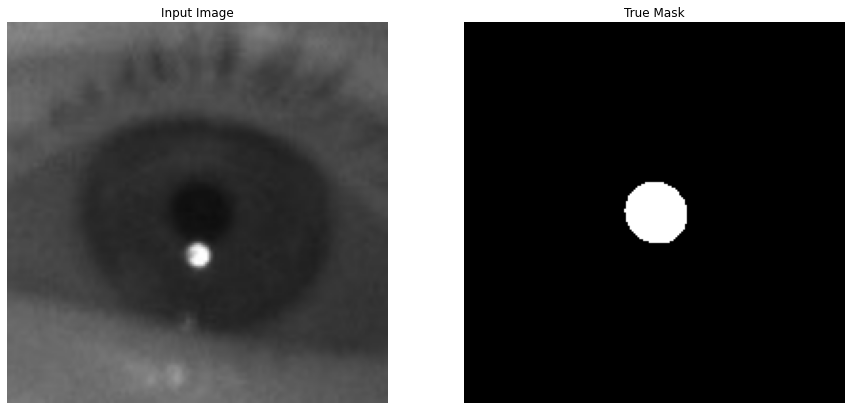
\includegraphics[width=0.8\linewidth]{input_image.png}
\caption{Пример входного изображения глаза и соответствующей маски зрачка.}
\label{fig:mpr}
\end{figure}

\begin{enumerate}
\item Дано растровое изображение в формате RGB, размером 200x200 пикселей и соответствующая ему маска зрачка (рис. 1).
\item Накладываем фильтр для сглаживание изображения Input Image по краям с использованием библиотеки OpenCV. Применяем метод GaussianBlur, что позволит нам избавиться от острых краев, броских деталей и различных шумов, сводя к минимуму чрезмерное размытие (рис. 2).

\begin{figure}[h]
\centering
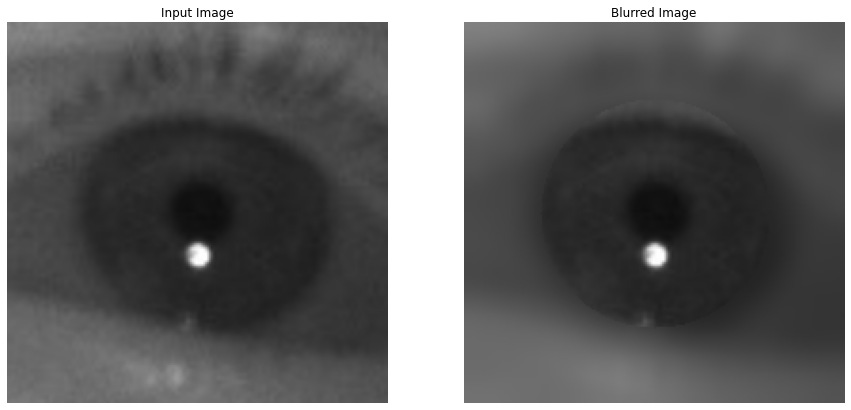
\includegraphics[width=0.8\linewidth]{blurred_image.png}
\caption{Размытие краев изображения с применением фильтра GaussianBlur.}
\label{fig:mpr}
\end{figure}

\item К предобработанному изображению Blurred Image применяем исследуемые алгоритмы: K-Means, DBSCAN и OPTICS (рис. 3). 
% Side by side subfigures 
\begin{figure}
\centering
\begin{subfigure}{0.8\linewidth}
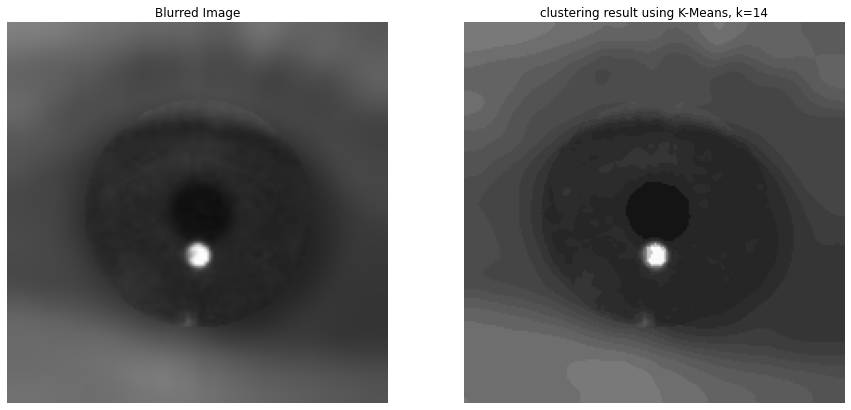
\includegraphics[width=\linewidth]{KMeans_results.png}
\end{subfigure}
\begin{subfigure}{0.8\linewidth}
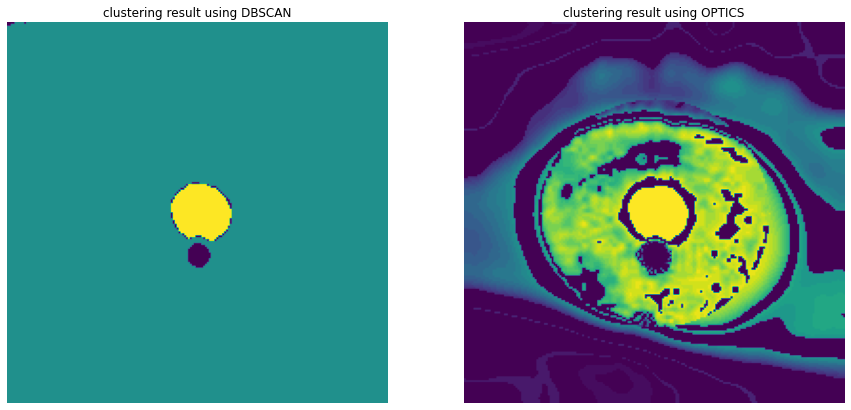
\includegraphics[width=\linewidth]{DBSCAN_OPTICS_results.png}
\end{subfigure}
\caption{Результаты кластеризации алгоритмов K-Means, DBSCAN и OPTICS.}
\label{fig:mpr}
\end{figure}


\item Выделяем только те пиксели, которые были отнесены к кластеру зрачка, тем самым формируя предсказанную маску Predicted Mask (рис. 4 - рис. 6). 

\item В качестве метрики качества рассмотрим Intersection over Union (IoU) - это число, которое количественно определяет степень перекрытия между двумя блоками. В случае сегментации объектов IoU оценивает перекрытие областей True Mask и Predicted Mask - отношение площади пересечения к объединенной площади предсказанного объекта и истинного.
\begin{equation}
IoU = \frac{ S_{Overlap}}{S_{Union}},
\end{equation}
где $S_{Overlap}$ - площадь пересечения True Mask и Predicted Mask; $S_{Union}$ - площадь объединения True Mask и Predicted Mask.

%----------------------------------
\begin{figure}
\centering
\begin{minipage}[c]{0.9\linewidth}
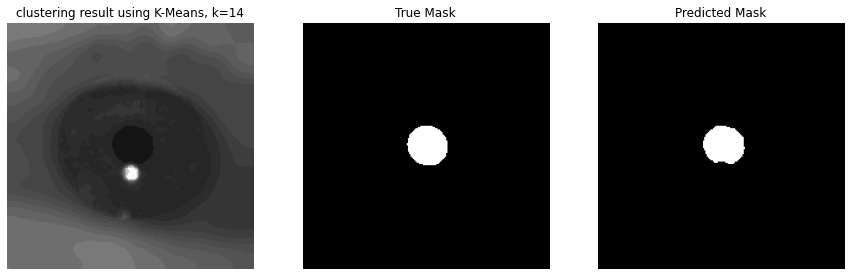
\includegraphics[width=\linewidth]{predicted_mask_KMeans.png}
\caption{Предсказанная маска зрачка, полученная в результате работы K-Means, IoU = 0.892.}
\end{minipage}

\begin{minipage}[c]{0.9\linewidth}
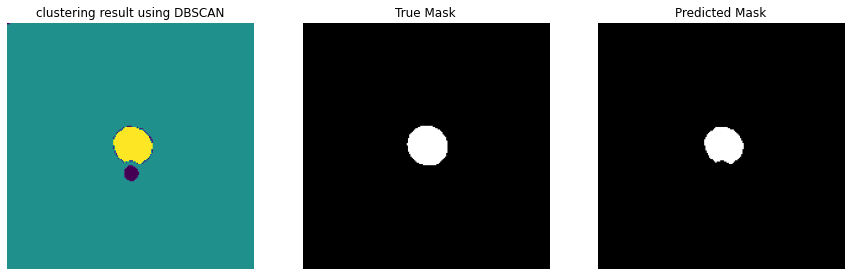
\includegraphics[width=\linewidth]{predicted_mask_DBSCAN.png}
\caption{Предсказанная маска зрачка, полученная в результате работы DBSCAN, IoU = 0.854.}
\end{minipage}

\begin{minipage}[c]{0.9\linewidth}
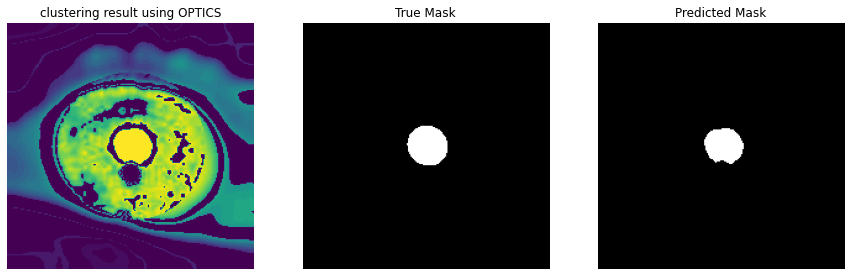
\includegraphics[width=\linewidth]{predicted_mask_OPTICS.png}
\caption{Предсказанная маска зрачка, полученная в результате работы OPTICS, IoU = 0.835.}
\end{minipage}
\label{fig:mpr}
\end{figure}
%----------------------------------


\item Применим описанную процедуру для датасета, содержащего 100 изображений, и рассмотрим средние значения метрик IoU для каждого алгоритма (таблица 1).

\begin{table}[H]
\centering
\caption{\label{tab:canonsummary} Средние показатели метрики качества IoU для алгоритмов K-Means, DBSCAN и OPTICS.}
\begin{tabular}{|c|p{4cm}|p{4cm}|}
\hline
Название метода & Среднее значение IoU для изображений без предпроцессинга & Среднее значение IoU для изображений с предпроцессингом \\
\hline
K-Means & $0.726$ & $0.750$\\
DBSCAN & $0.464$ & $0.735$ \\
OPTICS & $0.658$ & $0.623$\\
\hline
\end{tabular}
\end{table}


\end{enumerate}



\end{document}


